\documentclass[12pt,]{article}
\usepackage{lmodern}
\usepackage{amssymb,amsmath}
\usepackage{ifxetex,ifluatex}
\usepackage{fixltx2e} % provides \textsubscript
\ifnum 0\ifxetex 1\fi\ifluatex 1\fi=0 % if pdftex
  \usepackage[T1]{fontenc}
  \usepackage[utf8]{inputenc}
\else % if luatex or xelatex
  \ifxetex
    \usepackage{mathspec}
  \else
    \usepackage{fontspec}
  \fi
  \defaultfontfeatures{Ligatures=TeX,Scale=MatchLowercase}
\fi
% use upquote if available, for straight quotes in verbatim environments
\IfFileExists{upquote.sty}{\usepackage{upquote}}{}
% use microtype if available
\IfFileExists{microtype.sty}{%
\usepackage{microtype}
\UseMicrotypeSet[protrusion]{basicmath} % disable protrusion for tt fonts
}{}
\usepackage[margin=1in]{geometry}
\usepackage{hyperref}
\hypersetup{unicode=true,
            pdftitle={Linear Regression},
            pdfauthor={Jose Luis Contreras Santos, Antonio Javier González Ferrer, Alejandro González Pérez},
            pdfkeywords={pandoc, r markdown, knitr},
            pdfborder={0 0 0},
            breaklinks=true}
\urlstyle{same}  % don't use monospace font for urls
\usepackage{natbib}
\bibliographystyle{plainnat}
\usepackage{color}
\usepackage{fancyvrb}
\newcommand{\VerbBar}{|}
\newcommand{\VERB}{\Verb[commandchars=\\\{\}]}
\DefineVerbatimEnvironment{Highlighting}{Verbatim}{commandchars=\\\{\}}
% Add ',fontsize=\small' for more characters per line
\usepackage{framed}
\definecolor{shadecolor}{RGB}{248,248,248}
\newenvironment{Shaded}{\begin{snugshade}}{\end{snugshade}}
\newcommand{\KeywordTok}[1]{\textcolor[rgb]{0.13,0.29,0.53}{\textbf{{#1}}}}
\newcommand{\DataTypeTok}[1]{\textcolor[rgb]{0.13,0.29,0.53}{{#1}}}
\newcommand{\DecValTok}[1]{\textcolor[rgb]{0.00,0.00,0.81}{{#1}}}
\newcommand{\BaseNTok}[1]{\textcolor[rgb]{0.00,0.00,0.81}{{#1}}}
\newcommand{\FloatTok}[1]{\textcolor[rgb]{0.00,0.00,0.81}{{#1}}}
\newcommand{\ConstantTok}[1]{\textcolor[rgb]{0.00,0.00,0.00}{{#1}}}
\newcommand{\CharTok}[1]{\textcolor[rgb]{0.31,0.60,0.02}{{#1}}}
\newcommand{\SpecialCharTok}[1]{\textcolor[rgb]{0.00,0.00,0.00}{{#1}}}
\newcommand{\StringTok}[1]{\textcolor[rgb]{0.31,0.60,0.02}{{#1}}}
\newcommand{\VerbatimStringTok}[1]{\textcolor[rgb]{0.31,0.60,0.02}{{#1}}}
\newcommand{\SpecialStringTok}[1]{\textcolor[rgb]{0.31,0.60,0.02}{{#1}}}
\newcommand{\ImportTok}[1]{{#1}}
\newcommand{\CommentTok}[1]{\textcolor[rgb]{0.56,0.35,0.01}{\textit{{#1}}}}
\newcommand{\DocumentationTok}[1]{\textcolor[rgb]{0.56,0.35,0.01}{\textbf{\textit{{#1}}}}}
\newcommand{\AnnotationTok}[1]{\textcolor[rgb]{0.56,0.35,0.01}{\textbf{\textit{{#1}}}}}
\newcommand{\CommentVarTok}[1]{\textcolor[rgb]{0.56,0.35,0.01}{\textbf{\textit{{#1}}}}}
\newcommand{\OtherTok}[1]{\textcolor[rgb]{0.56,0.35,0.01}{{#1}}}
\newcommand{\FunctionTok}[1]{\textcolor[rgb]{0.00,0.00,0.00}{{#1}}}
\newcommand{\VariableTok}[1]{\textcolor[rgb]{0.00,0.00,0.00}{{#1}}}
\newcommand{\ControlFlowTok}[1]{\textcolor[rgb]{0.13,0.29,0.53}{\textbf{{#1}}}}
\newcommand{\OperatorTok}[1]{\textcolor[rgb]{0.81,0.36,0.00}{\textbf{{#1}}}}
\newcommand{\BuiltInTok}[1]{{#1}}
\newcommand{\ExtensionTok}[1]{{#1}}
\newcommand{\PreprocessorTok}[1]{\textcolor[rgb]{0.56,0.35,0.01}{\textit{{#1}}}}
\newcommand{\AttributeTok}[1]{\textcolor[rgb]{0.77,0.63,0.00}{{#1}}}
\newcommand{\RegionMarkerTok}[1]{{#1}}
\newcommand{\InformationTok}[1]{\textcolor[rgb]{0.56,0.35,0.01}{\textbf{\textit{{#1}}}}}
\newcommand{\WarningTok}[1]{\textcolor[rgb]{0.56,0.35,0.01}{\textbf{\textit{{#1}}}}}
\newcommand{\AlertTok}[1]{\textcolor[rgb]{0.94,0.16,0.16}{{#1}}}
\newcommand{\ErrorTok}[1]{\textcolor[rgb]{0.64,0.00,0.00}{\textbf{{#1}}}}
\newcommand{\NormalTok}[1]{{#1}}
\usepackage{graphicx,grffile}
\makeatletter
\def\maxwidth{\ifdim\Gin@nat@width>\linewidth\linewidth\else\Gin@nat@width\fi}
\def\maxheight{\ifdim\Gin@nat@height>\textheight\textheight\else\Gin@nat@height\fi}
\makeatother
% Scale images if necessary, so that they will not overflow the page
% margins by default, and it is still possible to overwrite the defaults
% using explicit options in \includegraphics[width, height, ...]{}
\setkeys{Gin}{width=\maxwidth,height=\maxheight,keepaspectratio}
\IfFileExists{parskip.sty}{%
\usepackage{parskip}
}{% else
\setlength{\parindent}{0pt}
\setlength{\parskip}{6pt plus 2pt minus 1pt}
}
\setlength{\emergencystretch}{3em}  % prevent overfull lines
\providecommand{\tightlist}{%
  \setlength{\itemsep}{0pt}\setlength{\parskip}{0pt}}
\setcounter{secnumdepth}{0}
% Redefines (sub)paragraphs to behave more like sections
\ifx\paragraph\undefined\else
\let\oldparagraph\paragraph
\renewcommand{\paragraph}[1]{\oldparagraph{#1}\mbox{}}
\fi
\ifx\subparagraph\undefined\else
\let\oldsubparagraph\subparagraph
\renewcommand{\subparagraph}[1]{\oldsubparagraph{#1}\mbox{}}
\fi

%%% Use protect on footnotes to avoid problems with footnotes in titles
\let\rmarkdownfootnote\footnote%
\def\footnote{\protect\rmarkdownfootnote}

%%% Change title format to be more compact
\usepackage{titling}

% Create subtitle command for use in maketitle
\newcommand{\subtitle}[1]{
  \posttitle{
    \begin{center}\large#1\end{center}
    }
}

\setlength{\droptitle}{-2em}
  \title{Linear Regression}
  \pretitle{\vspace{\droptitle}\centering\huge}
  \posttitle{\par}
  \author{Jose Luis Contreras Santos, Antonio Javier González Ferrer, Alejandro
González Pérez}
  \preauthor{\centering\large\emph}
  \postauthor{\par}
  \predate{\centering\large\emph}
  \postdate{\par}
  \date{enero, 2017}

\usepackage{bm}

\begin{document}
\maketitle
\begin{abstract}
An attempt to use linear regression to predict wine quality.
\end{abstract}

\section{Introduction}\label{introduction}

The aim of this section is to use linear regression to try and predict a
wine's quality based on its chemical attributes. To do this, we will
consider quality as a continuous variable ranging from 0 to 10. It is
worth noting, however, that this variable is in fact a categorical one
which can only take one of the 11 integer values comprised between 0 and
10. Therefore, as predictions will be continuous, many of them will most
likely be slightly off due to this discrepancy. This should not pose a
problem, however, as the usual error metrics, such as RMSE, can be
obtained anyways.

\section{Model fitting}\label{model-fitting}

After splitting the data in training and test sets, the training set was
used to fit a linear regression model. At first, all variables were used
as explanatory variables for the model.

\begin{Shaded}
\begin{Highlighting}[]
\CommentTok{# Train and test dataset, split 80% (data has been shuffled previously, no need to sample randomly)}
\NormalTok{split =}\StringTok{ }\KeywordTok{nrow}\NormalTok{(df)*}\FloatTok{0.8}
\NormalTok{train =}\StringTok{ }\NormalTok{df[}\DecValTok{1}\NormalTok{:split,]}
\NormalTok{test =}\StringTok{ }\NormalTok{df[split:}\KeywordTok{nrow}\NormalTok{(df),]}

\CommentTok{# Fit the model using all variables}
\NormalTok{model1 =}\StringTok{ }\KeywordTok{lm}\NormalTok{(quality~fixed_acidity+volatile_acidity+citic_acid}
            \NormalTok{+residual_sugar+chlorides+free_sulfur_dioxide}
            \NormalTok{+total_sulfur_dioxide+density+pH+sulphates+alcohol, }\DataTypeTok{data=}\NormalTok{train)}
\KeywordTok{summary}\NormalTok{(model1)}
\end{Highlighting}
\end{Shaded}

\begin{verbatim}
## 
## Call:
## lm(formula = quality ~ fixed_acidity + volatile_acidity + citic_acid + 
##     residual_sugar + chlorides + free_sulfur_dioxide + total_sulfur_dioxide + 
##     density + pH + sulphates + alcohol, data = train)
## 
## Residuals:
##     Min      1Q  Median      3Q     Max 
## -3.8027 -0.4544 -0.0414  0.4593  2.7242 
## 
## Coefficients:
##                        Estimate Std. Error t value Pr(>|t|)    
## (Intercept)           5.556e+01  1.399e+01   3.973 7.21e-05 ***
## fixed_acidity         6.376e-02  1.793e-02   3.556 0.000380 ***
## volatile_acidity     -1.304e+00  8.613e-02 -15.136  < 2e-16 ***
## citic_acid           -1.199e-01  8.904e-02  -1.347 0.178173    
## residual_sugar        4.162e-02  5.878e-03   7.080 1.64e-12 ***
## chlorides            -4.269e-01  3.602e-01  -1.185 0.236015    
## free_sulfur_dioxide   6.192e-03  8.400e-04   7.371 1.96e-13 ***
## total_sulfur_dioxide -2.547e-03  3.093e-04  -8.236 2.23e-16 ***
## density              -5.481e+01  1.427e+01  -3.842 0.000124 ***
## pH                    4.673e-01  1.028e-01   4.546 5.59e-06 ***
## sulphates             7.452e-01  8.423e-02   8.847  < 2e-16 ***
## alcohol               2.663e-01  1.957e-02  13.609  < 2e-16 ***
## ---
## Signif. codes:  0 '***' 0.001 '**' 0.01 '*' 0.05 '.' 0.1 ' ' 1
## 
## Residual standard error: 0.7338 on 5184 degrees of freedom
## Multiple R-squared:  0.2918, Adjusted R-squared:  0.2903 
## F-statistic: 194.1 on 11 and 5184 DF,  p-value: < 2.2e-16
\end{verbatim}

However, as the summary above indicates, the p-values for citic acid and
chlorides are not low enough to reject the null hypothesis. Thus, we can
consider that the contribution of these to the variance of quality is
not significantly greater than 0, and so they have been removed from the
final model. The resulting linear regression model is described below.

\begin{Shaded}
\begin{Highlighting}[]
\CommentTok{# Citic_acid removed from the model}
\NormalTok{model1 =}\StringTok{ }\KeywordTok{update}\NormalTok{(model1, ~.-citic_acid)}
\CommentTok{# Check if chlorides can also be removed}
\KeywordTok{summary}\NormalTok{(model1)}
\end{Highlighting}
\end{Shaded}

\begin{verbatim}
## 
## Call:
## lm(formula = quality ~ fixed_acidity + volatile_acidity + residual_sugar + 
##     chlorides + free_sulfur_dioxide + total_sulfur_dioxide + 
##     density + pH + sulphates + alcohol, data = train)
## 
## Residuals:
##     Min      1Q  Median      3Q     Max 
## -3.7891 -0.4580 -0.0373  0.4598  2.7323 
## 
## Coefficients:
##                        Estimate Std. Error t value Pr(>|t|)    
## (Intercept)           5.554e+01  1.399e+01   3.971 7.26e-05 ***
## fixed_acidity         5.809e-02  1.743e-02   3.333 0.000866 ***
## volatile_acidity     -1.259e+00  7.940e-02 -15.852  < 2e-16 ***
## residual_sugar        4.136e-02  5.876e-03   7.038 2.20e-12 ***
## chlorides            -5.103e-01  3.549e-01  -1.438 0.150475    
## free_sulfur_dioxide   6.232e-03  8.395e-04   7.424 1.33e-13 ***
## total_sulfur_dioxide -2.614e-03  3.053e-04  -8.563  < 2e-16 ***
## density              -5.479e+01  1.427e+01  -3.840 0.000124 ***
## pH                    4.770e-01  1.025e-01   4.652 3.38e-06 ***
## sulphates             7.409e-01  8.417e-02   8.801  < 2e-16 ***
## alcohol               2.642e-01  1.951e-02  13.544  < 2e-16 ***
## ---
## Signif. codes:  0 '***' 0.001 '**' 0.01 '*' 0.05 '.' 0.1 ' ' 1
## 
## Residual standard error: 0.7339 on 5185 degrees of freedom
## Multiple R-squared:  0.2915, Adjusted R-squared:  0.2901 
## F-statistic: 213.3 on 10 and 5185 DF,  p-value: < 2.2e-16
\end{verbatim}

\begin{Shaded}
\begin{Highlighting}[]
\CommentTok{# It can indeed be removed, do it}
\NormalTok{model1 =}\StringTok{ }\KeywordTok{update}\NormalTok{(model1, ~.-chlorides)}
\KeywordTok{summary}\NormalTok{(model1)}
\end{Highlighting}
\end{Shaded}

\begin{verbatim}
## 
## Call:
## lm(formula = quality ~ fixed_acidity + volatile_acidity + residual_sugar + 
##     free_sulfur_dioxide + total_sulfur_dioxide + density + pH + 
##     sulphates + alcohol, data = train)
## 
## Residuals:
##     Min      1Q  Median      3Q     Max 
## -3.7877 -0.4560 -0.0367  0.4578  2.7385 
## 
## Coefficients:
##                        Estimate Std. Error t value Pr(>|t|)    
## (Intercept)           5.958e+01  1.370e+01   4.348 1.40e-05 ***
## fixed_acidity         6.160e-02  1.726e-02   3.569 0.000362 ***
## volatile_acidity     -1.275e+00  7.863e-02 -16.211  < 2e-16 ***
## residual_sugar        4.318e-02  5.738e-03   7.526 6.15e-14 ***
## free_sulfur_dioxide   6.185e-03  8.390e-04   7.372 1.94e-13 ***
## total_sulfur_dioxide -2.576e-03  3.042e-04  -8.469  < 2e-16 ***
## density              -5.899e+01  1.397e+01  -4.224 2.44e-05 ***
## pH                    5.068e-01  1.004e-01   5.046 4.67e-07 ***
## sulphates             7.161e-01  8.240e-02   8.690  < 2e-16 ***
## alcohol               2.637e-01  1.951e-02  13.517  < 2e-16 ***
## ---
## Signif. codes:  0 '***' 0.001 '**' 0.01 '*' 0.05 '.' 0.1 ' ' 1
## 
## Residual standard error: 0.7339 on 5186 degrees of freedom
## Multiple R-squared:  0.2912, Adjusted R-squared:   0.29 
## F-statistic: 236.8 on 9 and 5186 DF,  p-value: < 2.2e-16
\end{verbatim}

According to the obtained model, the two variables with the highest
influence on quality are volatile acidity and density, specially the
latter. This can be misleading however, as it represents the variation
in quality per unit of the input, and the scales of the input variables
differ in their order of magnitude. Checking the distribution of
\(density\), for example, the difference between the maximum and minimun
values is lower than 0.03, whereas \(total_sulfur_dioxide\) has a range
of over 400. In any case, some conclusions can be extracted from this
output. For example, denser wines tend to have a higher perceived
quality, and the same happens to those with higher alcohol contents.

The adjusted R-squared coefficient of the resulting model is rather low,
with a value of only 0.29. Its associated p-value, however, is low
enough for us to be confident that there exists a relationship between
at least part of the input and the output variable, \(quality\).

\section{Assessing the model:
assumptions}\label{assessing-the-model-assumptions}

Let us further examine the quality of the linear regression model by
checking if the assumptions are met. In particular, we are interested in
testing if the residuals are independent, normal and have constant
variance.

\begin{Shaded}
\begin{Highlighting}[]
\CommentTok{# A: Check the assumptions}
\CommentTok{# Test normality}
\KeywordTok{jarque.bera.test}\NormalTok{(}\KeywordTok{residuals}\NormalTok{(model1)) }\CommentTok{# Answer: No normality}
\end{Highlighting}
\end{Shaded}

\begin{verbatim}
## 
##  Jarque Bera Test
## 
## data:  residuals(model1)
## X-squared = 287.77, df = 2, p-value < 2.2e-16
\end{verbatim}

\begin{Shaded}
\begin{Highlighting}[]
\CommentTok{# Equal variances}
\KeywordTok{bptest}\NormalTok{(model1) }\CommentTok{# No constant variance}
\end{Highlighting}
\end{Shaded}

\begin{verbatim}
## 
##  studentized Breusch-Pagan test
## 
## data:  model1
## BP = 79.793, df = 9, p-value = 1.777e-13
\end{verbatim}

\begin{Shaded}
\begin{Highlighting}[]
\CommentTok{# Testing independence of the residuals}
\KeywordTok{Box.test}\NormalTok{(}\KeywordTok{residuals}\NormalTok{(model1)) }\CommentTok{# Independent}
\end{Highlighting}
\end{Shaded}

\begin{verbatim}
## 
##  Box-Pierce test
## 
## data:  residuals(model1)
## X-squared = 0.1241, df = 1, p-value = 0.7246
\end{verbatim}

The conducted tests have different results. On the one hand, the
Box-Pierce test returns a high p-value, sign that there is not enough
evidence to reject the null hypothesis of independence. The results for
the Jarque-Bera and Breusch-Pagan tests, on the other hand, are not so
positive. According to their results, residuals are neither normal nor
homoscedastic.

\begin{figure}

{\centering 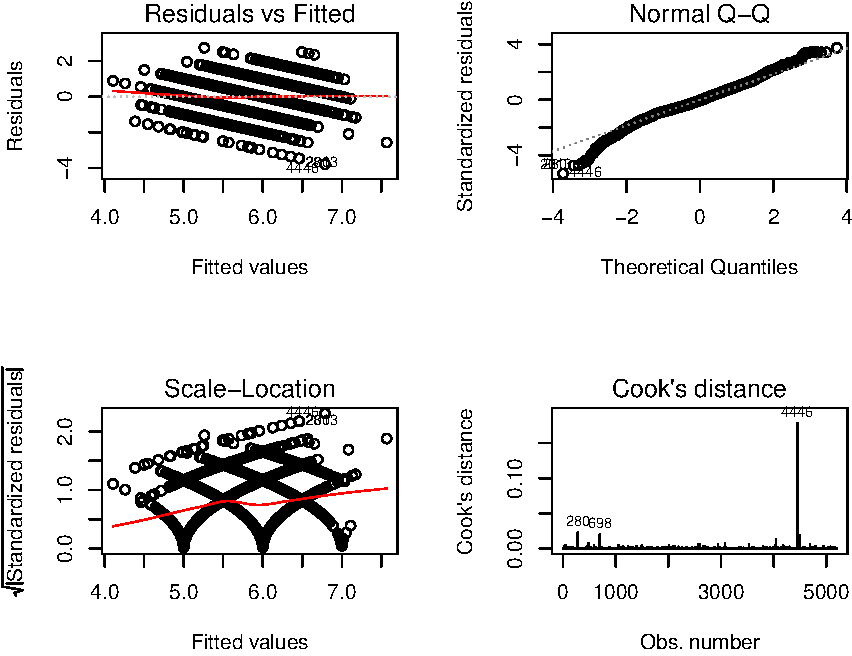
\includegraphics{quality-regression_files/figure-latex/residualplot-1} 

}

\caption{Residual plot}\label{fig:residualplot}
\end{figure}

Although the residual plots are unusual due to the clustering around the
integer values, they confirm the previous results. The Normal Q-Q plot
is in line with the results of the Jarque-Bera test, showing departures
from normality, specially in the first quartiles. From the Cook's
distance plot, a significant outlier can be seen, corresponding to
observation 4446.

\section{Evaluation of results}\label{evaluation-of-results}

\begin{Shaded}
\begin{Highlighting}[]
\CommentTok{# Residuals}
\KeywordTok{par}\NormalTok{(}\DataTypeTok{mfrow=}\KeywordTok{c}\NormalTok{(}\DecValTok{2}\NormalTok{,}\DecValTok{2}\NormalTok{))}
\KeywordTok{plot}\NormalTok{(model1, }\DataTypeTok{which=}\KeywordTok{c}\NormalTok{(}\DecValTok{1}\NormalTok{:}\DecValTok{4}\NormalTok{), }\DataTypeTok{ask=}\NormalTok{F)}
\end{Highlighting}
\end{Shaded}

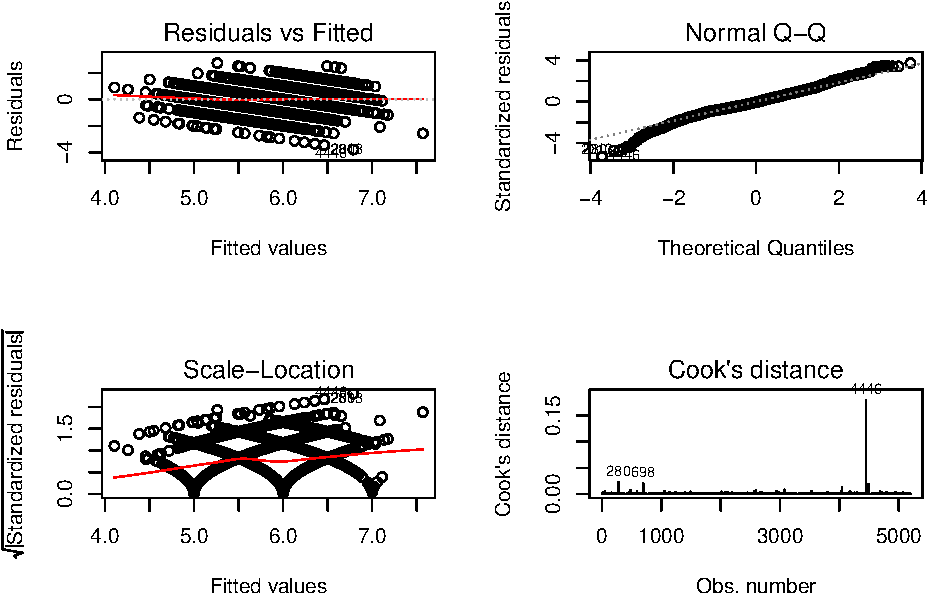
\includegraphics{quality-regression_files/figure-latex/evaluation-1.pdf}

\begin{Shaded}
\begin{Highlighting}[]
\CommentTok{# Un ojo a ese outlier gigante}

\CommentTok{# Conclusiones: en cuanto a hipotesis nuestro modelo es bastante mierda. Ademas parece que esta bien}
\CommentTok{# para qualitys entre 4 y 6 mas o menos, los valores mas grandes van mal. Esto es normal porque la}
\CommentTok{# muestra que tenemos es bastante mala (hacer histograma)}

\CommentTok{# 2. Assess the model. B: Evaluate performance}
\NormalTok{predicted <-}\StringTok{ }\KeywordTok{predict}\NormalTok{(model1, test)}

\CommentTok{# Percentage of correct predictions aka accuracy (we are rounding the predicted variable)}
\CommentTok{# Around 50% are correct - not bad}
\KeywordTok{sum}\NormalTok{(test$quality ==}\StringTok{ }\KeywordTok{round}\NormalTok{(predicted))/}\KeywordTok{nrow}\NormalTok{(test)}
\end{Highlighting}
\end{Shaded}

\begin{verbatim}
## [1] 0.5146154
\end{verbatim}

\begin{Shaded}
\begin{Highlighting}[]
\CommentTok{# But the above is a simplification, we are treating quality as a continuous var, so lets check}
\CommentTok{# more conventional metrics, in this case rmse}
\NormalTok{rmse <-}\StringTok{ }\NormalTok{(}\KeywordTok{sqrt}\NormalTok{(}\KeywordTok{mean}\NormalTok{(test$quality -}\StringTok{ }\NormalTok{predicted)^}\DecValTok{2}\NormalTok{))}
\NormalTok{rmse}
\end{Highlighting}
\end{Shaded}

\begin{verbatim}
## [1] 0.006010179
\end{verbatim}

\begin{Shaded}
\begin{Highlighting}[]
\CommentTok{# Pseudo rmse (after discretizing the output var by rounding)}
\CommentTok{# Aumenta bastante, pero ahora - yo diria - es una cifra mas indicativa}
\NormalTok{rmse.discret <-}\StringTok{ }\NormalTok{(}\KeywordTok{sqrt}\NormalTok{(}\KeywordTok{mean}\NormalTok{((test$quality -}\StringTok{ }\KeywordTok{round}\NormalTok{(predicted))^}\DecValTok{2}\NormalTok{)))}
\NormalTok{rmse.discret}
\end{Highlighting}
\end{Shaded}

\begin{verbatim}
## [1] 0.8133501
\end{verbatim}

\begin{Shaded}
\begin{Highlighting}[]
\CommentTok{# Conclusiones: No funciona mal en cuanto a resultados, pero no nos fiamos, entre que los}
\CommentTok{# datos son malillos (en cuanto a distribucion) y que no hemos usado la tecnica adecuada (ver abajo)}
\CommentTok{# En cualquier caso, posiblemente seria mejor usar Logistic Regression (o algun metodo de clasificacion)}
\CommentTok{# para predecir la quality, que realmente no es continua.}
\end{Highlighting}
\end{Shaded}


\end{document}
